\documentclass[UTF8]{ctexart}
\usepackage{hyperref}
\usepackage{abstract}
\usepackage[margin=1in]{geometry}
\usepackage{graphicx}
\begin{document}

\title{光的折射及色散曲线的测量}
\author{2019012137  物理92  张鸿琳}
\maketitle
\begin{abstract}
本实验主要探究光在不同介质中由于折射率不同引起的色散现象。首先通过分析,可知临界条件下,即偏转角度最小时,最小偏转角度与三棱镜的顶角以及折射率存在关系,通过该关系,只要找到最小偏转角度,就可以方便地测量出折射率,进而将一系列不同波长的光的折射率相互比较,处理数据得到色散曲线,以及阿贝数,从而更深刻地认识到该材料的折射能力,以及波长与折射率的关系。通过该实验,定量地了解了色散曲线和阿贝数,同时增强了自己处理数据的能力。

\centering
\textbf{Keywords:}折射率,色散曲线,偏转角度,阿贝数
\end{abstract}

\newpage
\tableofcontents
\newpage

\section{数据处理}
\subsubsection{公式推导}
由公式$n=\frac{sini}{sinr}=\frac{sin\frac{A+\delta}{2}}{sin\frac{A}{2}}$,得到$U_n$与$U_A$,$U_\delta$的关系为,$U_n=\sqrt{\frac{sin^2\frac{\delta}{2}}{4sin^4\frac{A}{2}}U_A^2+\frac{cos^2\frac{A+\delta}{2}}{4sin^2\frac{A}{2}}U_\delta^2}$。
\subsubsection{测量思路}
固定光源,使激光保持水平,旋转三棱镜,不断调节,直到左侧入射面上入射激光的反射光线和在棱镜中反射一周出射的光线平行(或者将光源改为多个平行光束,从而更好判定平行,具体现象见下图),由几何关系可得此时,偏转角最小,测量右侧出射光线偏离水平的角度即可。
\begin{center} 

\includegraphics[width=0.95\textwidth]{A.png} 
\end{center}
\begin{center} 

\includegraphics[width=0.95\textwidth]{B.png} 
\end{center}
\subsubsection{所得测量数据的处理}
(原始数据见“原始测量数据”)利用推导得到的公式以及原始数据,处理得到下表:
\begin{table}[h] 
\centering 
\begin{tabular}{|c|c|c|} 
\hline 
波长$\lambda$(nm) &  水棱镜中的折射率$n_w$ &玻璃棱镜中的折射率$n_g$ \\ 
\hline 
380 & 1.344733615 &1.518542615\\ 
\hline 
444 & 1.340853238 &1.510563625\\ 
\hline 
508 & 1.336963671  &1.505978875\\ 
\hline 
572 & 1.334365534  &1.502528267\\ 
\hline 
636 & 1.333064940 &1.500222139\\ 
\hline 
700 & 1.331763332 &1.497911442 \\ 
\hline
\end{tabular} 
\end{table}

波长为700nm时,已知$U_\delta=10'$,$U_A$=0,由推得的公式得,在水中测得的折射率不确定度为$U_{n_w}=\frac{cos\frac{A+\delta}{2}}{2sin\frac{A}{2}}U_\delta$=0.12,在玻璃中测得折射率不确定度为$U_{n_g}$=0.11。

已知在特定材料中波长与折射率满足$n_i=b_0+b_1\lambda_i^{-2.35}$,对数据进行处理并拟合,得到,在水中,满足方程$n_w=1.327932747+20055.78735\lambda^{-2.35}$,标准差为$s_{b_0}$=0.000515643,$s_{b_1}$=1024.079666,相对标准差为$\frac{s_{b_0}}{b_0}$=0.000388305,$\frac{s_{b_1}}{b_1}$=0.051061554,在玻璃中,满足方程,$n_g=1.492150144+30685.31404\lambda^{-2.35}$,标准差为$s_{b_0}$=0.000344834,$s_{b_1}$=684.8479814,相对标准差为$\frac{s_{b_0}}{b_0}$=0.000231099,$\frac{s_{b_1}}{b_1}$=0.022318428。拟合曲线如下图(为方便拟合,横坐标为波长的-2.35次方):
\begin{figure} [h]
\centering
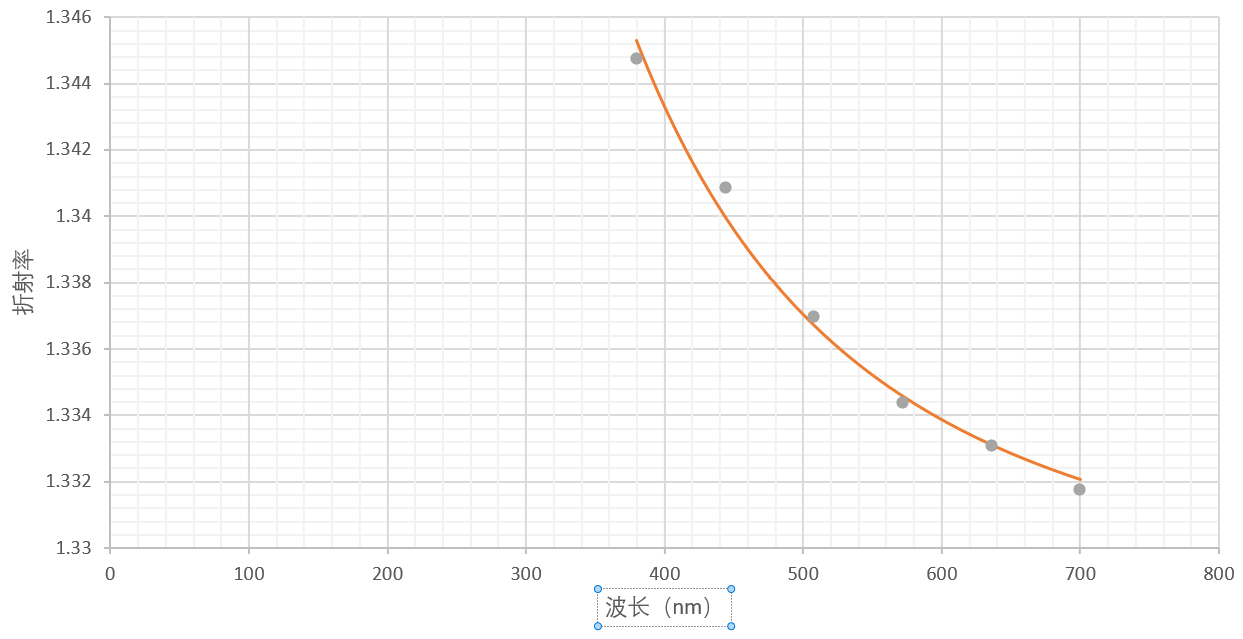
\includegraphics[width=0.95\textwidth]{C.png} 
\caption{水中的色散曲线}
\end{figure}
\begin{figure}[h] 
\centering
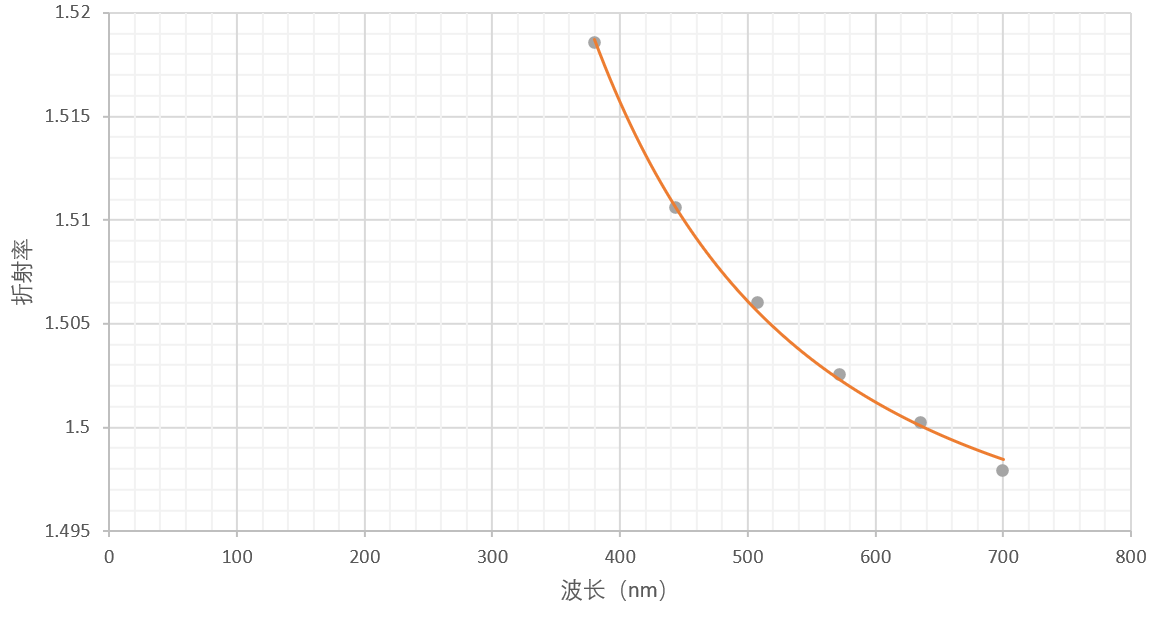
\includegraphics[width=0.95\textwidth]{D.png} 
\caption{玻璃中的色散曲线}
\end{figure}
\newpage
在水中,由色散曲线,可得$n_C$=1.3327422,$n_d$=1.334169621,$n_F$=1.337668544,阿贝数为$v_d=\frac{n_d-1}{n_F-n_C}=\frac{1.334169621-1}{1.337668544-1.3327422}$=67.83319003;在玻璃中,由色散曲线,可得$n_C$=1.499508598,$n_d$=1.501692549,$n_F$=1.507045894,阿贝数为$v_d=\frac{n_d-1}{n_F-n_C}=\frac{1.501692549-1}{1.507045894-1.499508598}$=66.56134203。
\section{讨论}
通过该实验,比较系统地了解了色散曲线以及阿贝数,但是仍有一些不足。比如,没有分析色散曲线的函数关系的由来,而是直接进行拟合,对现象地更深层次的认识就略有欠缺。另外,还可以做一些更细致的补充实验,使整个实验更加全面,比如,增加实验材料的种类,得到多条色散曲线,探究色散曲线系数的变化,同时还可以根据自己的猜想做一些假设,找出不同材料的不同点,探究不同材料色散能力或折射能力不同的根本原因,这样就使得整个实验更具有价值。

\section{原始测量数据}
\begin{table}[htbp!] 
\centering 
\begin{tabular}{|c|c|c|} 
\hline 
波长$\lambda$(nm) &  水棱镜中的最小偏转角$\delta_w$($^o$) &玻璃棱镜中的最小偏转角$\delta_g$($^o$) \\ 
\hline 
380 & 24.5 &38.8\\ 
\hline 
444 & 24.2 &38.1\\ 
\hline 
508 & 23.9  &37.7\\ 
\hline 
572 & 23.7  &37.4\\ 
\hline 
636 & 23.6  &37.2\\ 
\hline 
700 & 23.5 &37.0 \\ 
\hline
\end{tabular} 
\end{table}

\begin{thebibliography}{123456} 
\bibitem{ref1} 朱鹤年. 新概念基础物理实验讲义. 清华大学出版社. 2013. 
\bibitem{ref2} PhET:免费的在线物理、化学、生物、地理及数学仿真程序
\end{thebibliography}


\end{document}
